\section{Produtos Vetoriais em $\R^3$}

\begin{frame}[label=produtovetorial]{Produto Vetorial}

\begin{defin}
Sejam ${u}$ e ${v}$ vetores no espaço. O {\color{blue} produto vetorial} de ${u}$ por ${v}$, designado por ${u}\times {v}$, é o único vetor do espaço que satisfaz as seguinte condições:
\begin{enumerate}
	\item O {\color{blue} comprimento} é $\|\pv{u}{v}\|=\|{u}\|\ \|{v}\| \sin (\theta)$, onde $\theta$ é o ângulo entre $u$ e $v$;
	\item A {\color{blue} direção} é ortogonal a  ${u}$ e ${v}$ simultaneamente;
	\item O {\color{blue}sentido} dado pela regra da mão direita.
\end{enumerate}

Geometricamente, $\|u\times v\|$ representa a área do paralelogramo formado pelos representantes dos vetores $u$ e $v$ com mesma origem.
\end{defin}


\end{frame}



\begin{frame}[label=produtovetorial]{}
	
\begin{prop}
	Em um sistema de coordenadas, se $u=(u_1,u_2,u_3)$ e $v=(v_1,v_2,v_3)$, então 
	\[u\times v= 
	\left(
	\det \begin{bmatrix}
		u_2 & u_3\\
		v_2 & v_3
	\end{bmatrix},
	-\det \begin{bmatrix}
		u_1 & u_3\\
		v_1 & v_3
	\end{bmatrix},
	\det \begin{bmatrix}
		u_1 & u_2\\
		v_1 & v_2
	\end{bmatrix}
	\right)\]
\end{prop}
	
\begin{exe}
 Sejam $u=(1,2,3)$ e $v=(2,-1,1)$. Encontre $u\times v$.

\end{exe}

\end{frame}



\begin{frame}[label=produtovetorial]{}
	\begin{exe}
		Sejam $A=(1,-2,3)$, $B=(1,3,1)$ e $C=(1,-1,0)$. Calcule a área do paralelogramo que tem os segmentos $AB$ e $AC$ como arestas adjacente.
	\end{exe}
	
\begin{center}
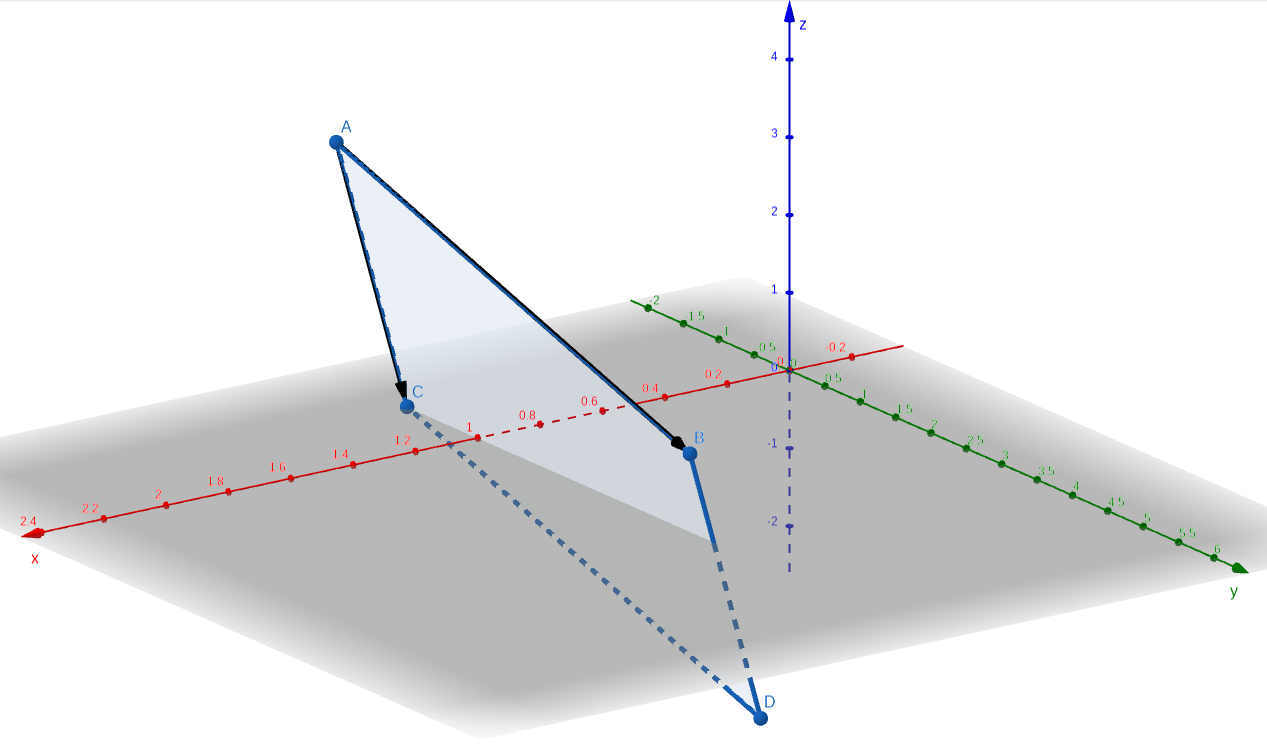
\includegraphics[scale=0.3]{figuras/paralelogramo.png}
\end{center}
	
\end{frame}


\begin{frame}[label=produtovetorial]{}
\begin{casa}
Determine a área do triângulo cujos vértices são os pontos $A=(3,2,0)$, $B=(1,0,2)$ e $C=(0,4,3)$.
\end{casa}
	
\end{frame}





\begin{frame}[label=produtovetorial]{}
\begin{block}{Propriedades do Produto Vetorial}
\begin{enumerate}
	\item $\|\pv{u}{v}\|=0\Leftrightarrow$ $u=0$ ou $v=0$ ou ${u}, {v}$ são múltiplos.
	\item $\pv{u}{v}=-\pv{v}{u}$  (anticomutatividade).
	\item $(\lambda {u})\times {v}={u}\times (\lambda{v})=\lambda(\pv{u}{v})$.
	\item ${u}\times({v}+{w})=\pv{u}{v}+\pv{u}{w}$.
\end{enumerate}
\end{block}
\begin{exe}
Mostre que se $u+v+w=0$, então $u\times v=v\times w$.
\end{exe}
\end{frame}

\subsection*{Distância entre ponto e reta}

\begin{frame}[label=produtovetorial]{Aplicação: Distância de Ponto à reta}
Dados um ponto $A$ e uma reta $\ell$ no espaço. Então, a {\color{blue}distância entre $A$ e $\ell$ } é dada por 
\[{\color{red}d(A,\ell)=\frac{\|AP\times v\|}{\|v\|}},\]
onde $P$ é um ponto e $v$ um vetor diretor  de $\ell$.

\begin{exe}
	Achar a distância entre $A=(3,0,-2)$ e 
	$\ell:\begin{cases}
		x=1-t\\ y=2+2t\\ z=t,\ t\in \R.
	\end{cases}$
\end{exe}
	
\end{frame}


\begin{frame}[label=produtovetorial]{}
\begin{casa}
\begin{enumerate}
	\item Obtenha a reta $r$ dada pela inteseção dos planos $\pi_1: x+y+z=2$ e $\pi_2:x-y-z=0$.
	
	\item Determine os pontos da reta $r$ que estão à distância $\sqrt{6}$ da reta 
$s:\begin{cases}
	x=1+t\\ y=-t\\ z=-1+t,\ t\in \R.
\end{cases}$
\end{enumerate}
\end{casa}
	
\end{frame}

\begin{frame}[label=produtovetorial]{Produto Misto}
\begin{defin}
	O {\color{blue} produto misto} entre os vetores $u,v$ e $w$ em $\R^3$ é o número real
	\[[u,v,w]:=(u\times v)\cdot w.\]
	
Geometricamente $\left| [u,v,w]  \right|$ representa o volume do paralelepípedo cujas arestas são representantes dos vetores $u,v$ e $ w $ com mesma origem.
\end{defin}
	
\end{frame}





\begin{frame}[label=produtovetorial]{}
	
\begin{prop}
	Se $u=(u_1,u_2,u_3)$, $v=(v_1,v_2,v_3)$ e $w=(w_1,w_2,w_3)$, então
\[[u,v,w]=\det
\begin{bmatrix}
	u\\
	v\\
	w
\end{bmatrix}
\]
\end{prop}
\begin{exe}
Determinar o volume do paralelepípedo que tem por arestas adjacentes os segmentos $AB$, $AC$ e $AD$, onde $A=(1,0,1)$, $B=(0,1,1)$, $C=(1,1,1)$ e $D=(1,-1,-1)$.
\end{exe}
\end{frame}

\begin{frame}[label=produtovetorial]{}
\begin{casa}
	Determinar $x$ para que o volume do paralelepípedo que tem um dos vértices no ponto $A=(2,1,6)$ e os três vértices adjacentes nos pontos $B=(4,1,3)$, $C=(1,3,2)$ e $D=(1,x,1)$ seja igual a $15$.
\end{casa}
	
\end{frame}

\begin{frame}[label=produtovetorial]{Distância entre retas}



	
\end{frame}




